\documentclass[12pt]{article}
\usepackage[margin=1in]{geometry}
\usepackage{amsmath,amssymb,booktabs,graphicx,natbib,hyperref,xr}
\graphicspath{{figures/}}
\externaldocument[main-]{manuscript}
\newcommand{\cut}{\mathcal{C}}
\newcommand{\nnl}{\operatorname{NNL}}
\setlength{\tabcolsep}{4pt}
\title{Supplementary information: compressing dense similarity for dataset splitting}
\author{Author information pending}
\date{}
\begin{document}
\maketitle
\section{Dataset scope}

Target slices follow the declared dataset-loader mapping and supply one scalar
task per source for the prediction studies. Structural benchmarks optimize
features without using responses, including entities whose target is missing.
The study does not claim coverage of every target in Tox21, SIDER or MUV.
MUV-466 has sparse labels and few actives; no predictive AUC is reported for
MUV in this article. The dataset catalogue identifies the exact offline
snapshots rather than silently substituting a newer database query.
\begin{table}[htbp]\centering\small
\begin{tabular}{lrrp{2.5in}r}
\toprule
Dataset & Entities & Labelled & Target & Positive \\
\midrule
bace & 1513 & 1513 & Class & 691 \\
bbbp & 2039 & 2039 & p\_np & 1560 \\
esol & 1128 & 1128 & measured log solubility in mols per litre & -- \\
freesolv & 642 & 642 & expt & -- \\
lipophilicity & 4200 & 4200 & exp & -- \\
clintox & 1480 & 1480 & CT\_TOX & 112 \\
hiv & 41120 & 41120 & HIV\_active & 1443 \\
tox21 & 7823 & 7258 & NR-AR & 308 \\
sider & 1427 & 1427 & Hepatobiliary disorders & 743 \\
muv & 93087 & 14841 & MUV-466 & 27 \\
qm8 & 21786 & 21786 & E1-CC2 & -- \\
qmof & 20372 & 20372 & outputs.pbe.bandgap & -- \\
materials project & 100000 & 99998 & formation\_energy\_per\_atom & -- \\
\bottomrule
\end{tabular}
\caption{Retained entities, declared target slices and label coverage. Positive counts apply only to binary tasks; dashes denote continuous targets. Structural splitting retains valid features independently of missing responses. Single-target slices do not constitute an evaluation of all assays in a multitask source. Exact raw-file and retained-identity hashes accompany the catalogue.}\end{table}

\section{Settings and computational scope}

\begin{table}[htbp]\centering
\begin{tabular}{llll}
\toprule
Setting & Power & Group threshold & Capacity tolerance\\
\midrule
Plain & 1 & None & 0, 0.01 or 0.05\\
Power only & 3 & None & 0\\
Groups only & 1 & 0.4 & 0\\
Combined & 3 & 0.4 & 0, 0.01 or 0.05\\
Higher-threshold combined & 3 & 0.6 & 0.01 or 0.05\\
\bottomrule
\end{tabular}
\caption{Readable setting names. Standard factors have rank 256, four restarts
and at most 25 assignment iterations. Molecular thresholds refer to the
1024-bit radius-two Morgan/Tanimoto representation. Group caps are half the
smallest target fold, with the freeze rule; top-32 neighbours use exact CPU
blocks in the benchmark and exact GPU tiling in the H100 scaling study.
Materials grouping instead uses a representation-specific similarity quantile.}
\end{table}

\begin{table}[htbp]\centering
\begin{tabular}{ll}
\toprule
Operation & Storage or arithmetic scope\\
\midrule
Factor storage & $O(nr)$\\
Factor construction/whitening & $O(nrd+nr^2+r^3)$ arithmetic\\
Fold products, fixed fold count & $O(nr)$ per iteration, plus assignment sorting\\
$M$ point-refinement moves & Up to $O(Mnr)$ arithmetic\\
Exact neighbour construction & $O(n^2d)$ arithmetic; blocked temporary storage\\
Retained neighbour indices & $O(nk)$ storage\\
\bottomrule
\end{tabular}
\caption{Computational scope for $n$ entities, feature dimension $d$, rank $r$
and neighbour degree $k$. Input features and outputs occupy additional storage.
If the number of refinement moves grows with $n$, refinement can be quadratic.
The factor-storage statement alone is not a linear-time claim.}
\end{table}

\section{Factor construction and optimization details}

The main article presents the factor-space objective and its scientific use.
This section records the numerical choices needed to reproduce the solver.
The regularized landmark eigendecomposition floors eigenvalues at $10^{-6}$.

Landmark selection affects approximation fidelity; fixed and adaptive sampling
are established alternatives \citep{kumar2012,musco2017}. The implementation
supports uniform landmarks and a similarity-based spreading
heuristic historically named \texttt{kmeans++}. The latter samples proportional
to $(1-\max_j S_{ij})^2$ over current landmarks. This is not ordinary squared
Hilbert-distance sampling for a normalized kernel, so standard k-means++
initialization guarantees do not automatically apply. We retain its name for API
compatibility and evaluate uniform sampling as an ablation.


The target count for each fold is obtained by largest-remainder rounding.
For normalized requested fractions $q_c$, the tolerance corridor is based on
$(1\pm\epsilon)nq_c$, with integer bounds widened only enough to contain the
rounded target. Zero tolerance yields the exact integer targets.

Each restart starts from a seeded count-constrained assignment. The two-fold
linear subproblem is solved by sorting preference differences while enforcing
both folds' bounds. Three-fold assignment uses a regret-ordered greedy peel
that leaves sufficient capacity for the remaining folds. Proposals exclude
self-similarity and are accepted only when the sum of squared fold sums does
not decrease. A rejected proposal ends the restart. The best restart undergoes
move refinement, or size-preserving pair swaps at exact capacities. The current
fold is masked before alternative destinations are searched. Candidate limits
make this a local search. Point-level refinement is skipped above two million
entities. The standard settings are rank 256, four restarts and at most 25
assignment iterations.

For groups, the default freeze rule stops growth of the larger component after
a cap-blocked merge. The alternative skip rule rejects only that merge. Weighted
assignment and repair operate on group counts; groups dissolved into singletons
are counted in the output diagnostics. Failure to satisfy the final count
corridor raises an error. The multi-component extension concatenates per-axis
factors. Dense identity columns for repeated featureless values can make its
storage quadratic, so this extension is outside the reported scaling claims.

\section{Neighbour construction details}

The CPU reference scans exact similarities in row blocks. Blocking limits
temporary storage while retaining quadratic arithmetic. Two-dimensional GPU
tiling supplies a second exact backend. The optional NN-Descent candidate graph
over packed binary fingerprints recomputes retained Tanimoto similarities using
exact bit intersections. Its candidate recall is approximate. Top-32 recall and
recall of exact top-32 edges at similarity at least 0.4 use 256 uniformly sampled
query entities. Index-based recall is conservative when similarities tie.
Compilation warm-up is recorded separately from warm graph construction.
The retained graph-construction measurements appear below. Their split-quality
and optimizer clocks are not used to characterize the revised solver.
\begin{table}[htbp]\centering\small
\begin{tabular}{rlrrr}
\toprule
Entities & Backend & Graph seconds & Top-32 recall & Strong recall \\
\midrule
1000 & Exact tiled & 0.009 & 1.000 & 1.000 \\
10000 & Exact tiled & 0.240 & 1.000 & 1.000 \\
100000 & Exact tiled & 13.002 & 1.000 & 1.000 \\
30000 & Exact tiled & 1.287 & 1.000 & 1.000 \\
1000 & NN-Descent & 0.842 & 1.000 & 1.000 \\
10000 & NN-Descent & 8.132 & 0.993 & 1.000 \\
100000 & NN-Descent & 97.569 & 0.990 & 0.998 \\
30000 & NN-Descent & 26.129 & 0.994 & 1.000 \\
\bottomrule
\end{tabular}
\caption{Neighbour-graph engineering measurements on ChEMBL fingerprints. Exact tiled search uses a Tesla T4; NN-Descent uses two CPU threads. Recall is measured on 256 sampled query entities; strong recall restricts exact top-32 edges to similarity at least 0.4. ANN compilation warm-up is separate. These are graph-construction observations from the preserved source study, not H100 split-call timings or measurements of the revised partition optimizer.}\end{table}


\section{Powered-kernel fidelity and rank sensitivity}

The fidelity study uses six full datasets: FreeSolv, ESOL, BACE, BBBP, ClinTox
and Lipophilicity. For each power, rank and seed, a factor and optimized partition
are constructed with the release solver. Five count-preserving perturbations
give a spectrum of partitions evaluated against the same factor and exact
powered kernel. The tables distinguish empirical cut errors from the spectral
residual estimate. The latter is obtained with a symmetric eigensolver, a fixed
starting vector and tolerance $10^{-8}$; its eigenpair residual is retained in
the machine-readable results. It is not a certified numerical upper bound.

\begin{figure}[htbp]
\centering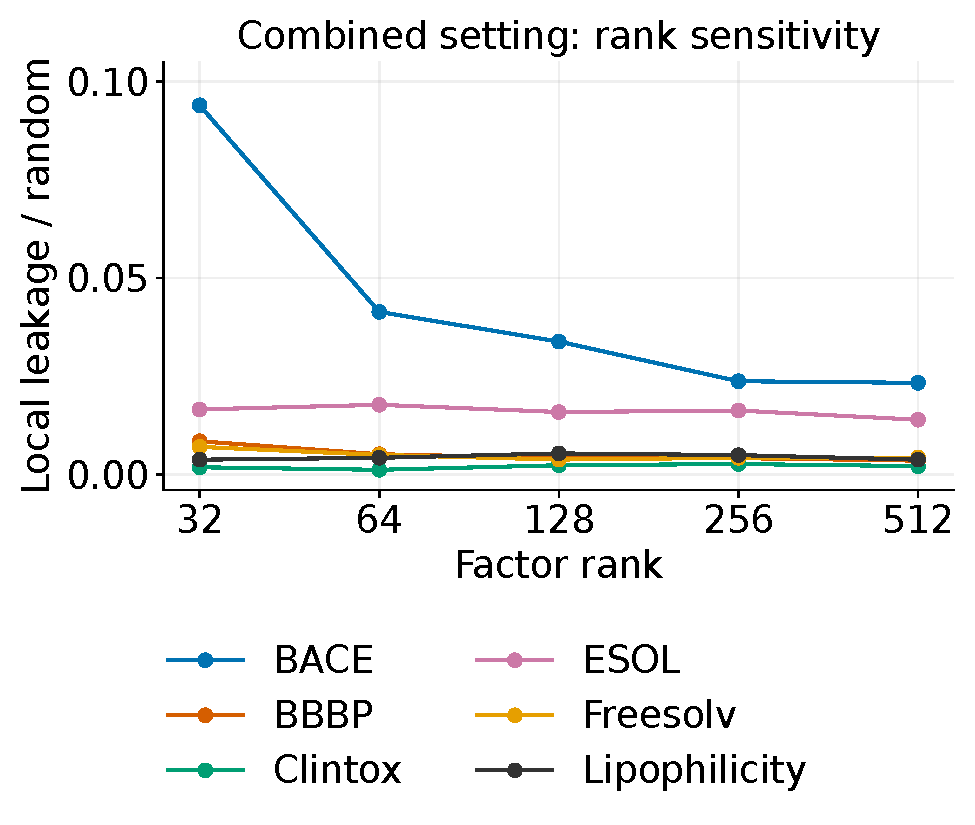
\includegraphics[width=6.5in]{revision/combined_rank.pdf}
\caption{Combined-setting local leakage versus rank. Values average three split
seeds at exact integer fold counts. Here local queries include validation and
test, for continuity with the rank study's stored metric. The main baseline
comparison uses test-only local queries and reports pooled held-out queries
separately. Small nonmonotone changes are retained.}
\end{figure}

\section{External assay sensitivity}

Original and class-balanced partitions share fold counts and input molecules.
Class-balanced assignments use target labels, and their structural composition
changes. They diagnose sensitivity and are not a proposed label-blind splitter.
Per-assay JSON records retain all assignments, input and producer hashes,
nearest-training-molecule similarity and label support, and all model scores.
Reported ROC-AUC below 0.5 is retained; no prediction is flipped after inspecting
the test labels. Class rates accompany AUC so shifts are visible directly.

\begin{figure}[htbp]
\centering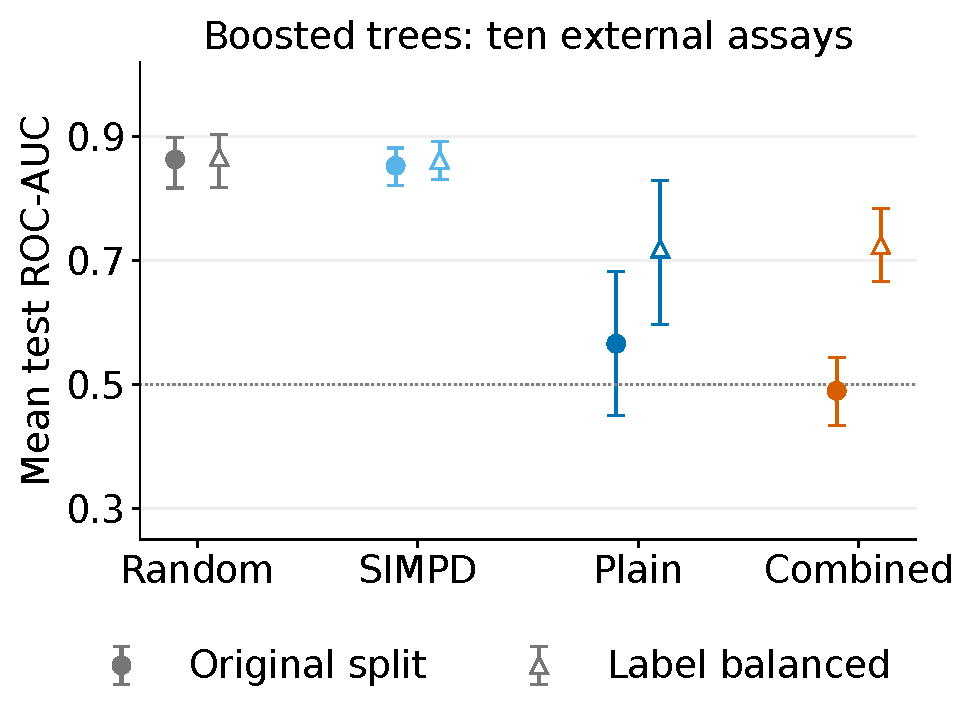
\includegraphics[width=6.5in]{revision/external_xgb.pdf}
\caption{Boosted-tree absolute AUC with the same protocol and assay-bootstrap
intervals as the main RF figure. Circles show original partitions; triangles
show the target-aware intervention.}
\end{figure}

\begin{table}[htbp]\centering\small
\begin{tabular}{rrrrr}
\toprule
Power & Rank & Max error / mass & Median bound / mass & Max bound / mass \\
\midrule
1 & 32 & 0.0808 & 0.4403 & 0.6789 \\
1 & 64 & 0.0369 & 0.2488 & 0.3695 \\
1 & 128 & 0.0164 & 0.1323 & 0.2451 \\
1 & 256 & 0.0058 & 0.0716 & 0.1191 \\
1 & 512 & 0.0021 & 0.0337 & 0.0569 \\
3 & 32 & 0.3110 & 3.3021 & 7.2872 \\
3 & 64 & 0.2788 & 3.1409 & 7.1525 \\
3 & 128 & 0.2239 & 2.6336 & 7.0219 \\
3 & 256 & 0.1563 & 2.1753 & 5.8603 \\
3 & 512 & 0.0958 & 1.4566 & 2.7974 \\
\bottomrule
\end{tabular}

\caption{Six full development datasets, three seeds and five partition perturbations per factor. Numerical spectral estimates use a symmetric eigensolver and are not certified upper bounds. Values above one give a vacuous bound on a cut ratio.}\end{table}
\begin{table}[htbp]\centering\small
\begin{tabular}{lrrrrr}
\toprule
Assay & Random & SIMPD & Plain & Combined & Balanced \\
\midrule
1293269-1 & 0.875 & 0.931 & 0.724 & 0.409 & 0.886 \\
1889-1 & 0.870 & 0.903 & 0.496 & 0.464 & 0.846 \\
225-1 & 0.784 & 0.848 & 0.534 & 0.525 & 0.583 \\
237-1 & 0.890 & 0.839 & 0.605 & 0.529 & 0.656 \\
269-1 & 0.933 & 0.887 & 0.500 & 0.384 & 0.867 \\
2820-1 & 0.900 & 0.903 & 0.439 & 0.416 & 0.815 \\
284-1 & 0.890 & 0.847 & 0.711 & 0.554 & 0.767 \\
3837-1 & 0.932 & 0.901 & 0.456 & 0.410 & 0.545 \\
3952-3 & 0.921 & 0.839 & 0.624 & 0.824 & 0.821 \\
4105864-1 & 0.713 & 0.767 & 0.801 & 0.706 & 0.781 \\
\bottomrule
\end{tabular}

\caption{RF mean test ROC-AUC by assay. Balanced refers to the combined partition after the target-aware intervention; it is not the label-blind method.}\end{table}
\begin{table}[htbp]\centering\small
\begin{tabular}{lrrrrr}
\toprule
Assay & Random & SIMPD & Plain & Combined & Balanced \\
\midrule
1293269-1 & 0.903 & 0.915 & 0.925 & 0.422 & 0.871 \\
1889-1 & 0.858 & 0.912 & 0.701 & 0.601 & 0.841 \\
225-1 & 0.795 & 0.849 & 0.476 & 0.596 & 0.663 \\
237-1 & 0.883 & 0.846 & 0.647 & 0.543 & 0.586 \\
269-1 & 0.927 & 0.867 & 0.512 & 0.499 & 0.776 \\
2820-1 & 0.899 & 0.878 & 0.380 & 0.322 & 0.756 \\
284-1 & 0.866 & 0.862 & 0.650 & 0.387 & 0.617 \\
3837-1 & 0.909 & 0.861 & 0.515 & 0.560 & 0.620 \\
3952-3 & 0.897 & 0.777 & 0.193 & 0.433 & 0.783 \\
4105864-1 & 0.693 & 0.759 & 0.661 & 0.538 & 0.736 \\
\bottomrule
\end{tabular}

\caption{XGB mean test ROC-AUC by assay. Balanced refers to the combined partition after the target-aware intervention; it is not the label-blind method.}\end{table}
\begin{table}[htbp]\centering\small
\begin{tabular}{lrr}
\toprule
Assay & Train positive rate & Test positive rate \\
\midrule
1293269-1 & 0.415 & 0.356 \\
1889-1 & 0.388 & 0.395 \\
225-1 & 0.387 & 0.359 \\
237-1 & 0.397 & 0.405 \\
269-1 & 0.418 & 0.362 \\
2820-1 & 0.403 & 0.396 \\
284-1 & 0.412 & 0.390 \\
3837-1 & 0.387 & 0.411 \\
3952-3 & 0.394 & 0.352 \\
4105864-1 & 0.389 & 0.451 \\
\bottomrule
\end{tabular}

\caption{Class proportions for random; averages over split seeds.}\end{table}
\begin{table}[htbp]\centering\small
\begin{tabular}{lrr}
\toprule
Assay & Train positive rate & Test positive rate \\
\midrule
1293269-1 & 0.417 & 0.350 \\
1889-1 & 0.374 & 0.453 \\
225-1 & 0.352 & 0.500 \\
237-1 & 0.370 & 0.514 \\
269-1 & 0.390 & 0.473 \\
2820-1 & 0.391 & 0.444 \\
284-1 & 0.388 & 0.486 \\
3837-1 & 0.429 & 0.242 \\
3952-3 & 0.363 & 0.479 \\
4105864-1 & 0.410 & 0.367 \\
\bottomrule
\end{tabular}

\caption{Class proportions for published simpd; averages over split seeds.}\end{table}
\begin{table}[htbp]\centering\small
\begin{tabular}{lrr}
\toprule
Assay & Train positive rate & Test positive rate \\
\midrule
1293269-1 & 0.429 & 0.300 \\
1889-1 & 0.374 & 0.453 \\
225-1 & 0.383 & 0.375 \\
237-1 & 0.433 & 0.257 \\
269-1 & 0.468 & 0.161 \\
2820-1 & 0.464 & 0.154 \\
284-1 & 0.401 & 0.433 \\
3837-1 & 0.386 & 0.414 \\
3952-3 & 0.391 & 0.366 \\
4105864-1 & 0.408 & 0.376 \\
\bottomrule
\end{tabular}

\caption{Class proportions for plain; averages over split seeds.}\end{table}
\begin{table}[htbp]\centering\small
\begin{tabular}{lrr}
\toprule
Assay & Train positive rate & Test positive rate \\
\midrule
1293269-1 & 0.333 & 0.683 \\
1889-1 & 0.392 & 0.380 \\
225-1 & 0.388 & 0.356 \\
237-1 & 0.419 & 0.315 \\
269-1 & 0.455 & 0.215 \\
2820-1 & 0.466 & 0.145 \\
284-1 & 0.400 & 0.438 \\
3837-1 & 0.382 & 0.431 \\
3952-3 & 0.430 & 0.211 \\
4105864-1 & 0.430 & 0.287 \\
\bottomrule
\end{tabular}

\caption{Class proportions for combined; averages over split seeds.}\end{table}

\clearpage
\section{Scaling measurements}

The plain-factor and exact-tiled combined pipelines use the same ChEMBL cache,
nested sample indices, kernel rank and two-thread CPU allocation. Independent
cases are distributed across reserved H100s, with one process per case. All
returned assignments satisfy the stated two-sided count corridor. The table
reports the actual measured ranges without extending the combined setting to
unmeasured sizes. Saved sample indices and assignments allow independent checks
of retention, counts and nesting.
\begin{table}[htbp]\centering\small
\begin{tabular}{lrrrr}
\toprule
Setting & Molecules & Seconds & GPU GiB & Host RSS GiB \\
\midrule
Plain & 1000 & 0.10 & 0.05 & 1.47 \\
Plain & 10000 & 0.32 & 0.16 & 2.12 \\
Plain & 100000 & 1.37 & 1.30 & 5.34 \\
Plain & 300000 & 3.55 & 3.83 & 11.86 \\
Plain & 1000000 & 10.83 & 12.67 & 34.70 \\
Plain & 2000000 & 19.93 & 25.32 & 67.34 \\
Combined & 1000 & 0.15 & 0.05 & 1.49 \\
Combined & 10000 & 1.67 & 0.16 & 2.13 \\
Combined & 30000 & 27.45 & 0.42 & 3.01 \\
Combined & 100000 & 89.04 & 1.30 & 5.33 \\
\bottomrule
\end{tabular}
\caption{Fresh-process H100 NVL scaling cases at rank 256 and size tolerance 0.01. Split time excludes feature loading and scoring and follows a 100-entity warm-up. GPU peak is reset after warm-up; process RSS includes inputs and warm-up. The combined setting uses exact tiled neighbours. These are single-seed measurements, not repeated timing distributions.}\end{table}

\clearpage
\section{Threshold and independent-representation robustness}

Power/threshold cases and their controls share the same retained rows and exact
8:1:1 integer targets. Morgan and MACCS kernels are scored exactly on the full
datasets, with test-only local queries and the complete training fold as
reference. Three random assignments at those counts supply a common
normalization for all settings within a seed. MACCS keys are never supplied to
the optimizer. Its raw nearest-neighbour similarity is the primary independent
representation check: the absolute Morgan ramp cutoffs have no universal
interpretation for MACCS.

\begin{figure}[htbp]
\centering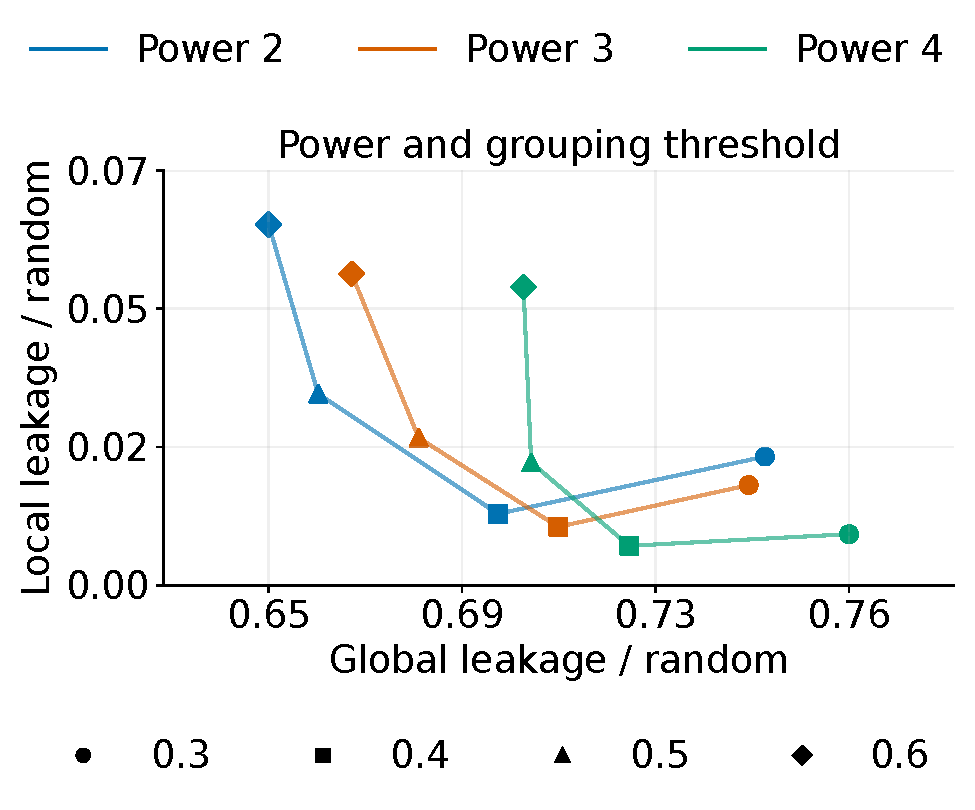
\includegraphics[width=6.5in]{revision/power_threshold_frontier.pdf}
\caption{Power/threshold sensitivity at exact fold counts on six full
development datasets. Each point averages dataset means after averaging three
split seeds. Colours denote kernel power; marker shapes denote grouping
thresholds, listed along the bottom. Lines connect thresholds in increasing
order within each power. Both axes use the original Morgan kernel; local
queries are test-only. The settings were not selected using external-assay
prediction scores.}
\end{figure}


\begin{figure}[htbp]
\centering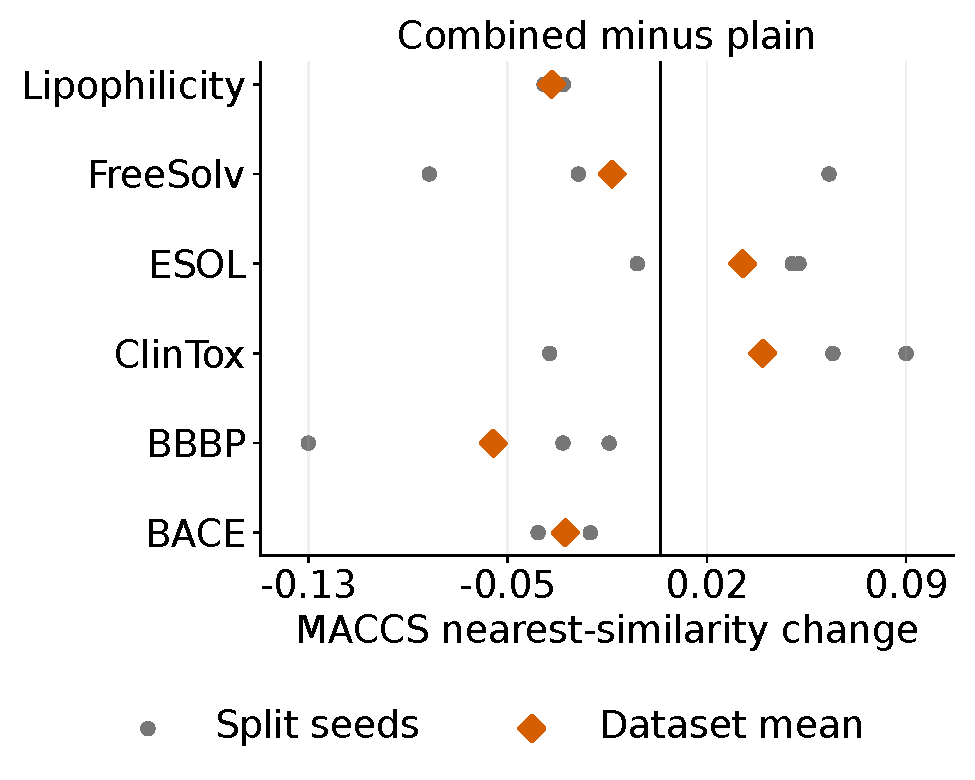
\includegraphics[width=6.5in]{revision/independent_fingerprint.pdf}
\caption{MACCS nearest-training-similarity changes for the fixed combined
setting relative to plain low rank. Small circles are paired split-seed
differences and diamonds are dataset means. Negative values indicate lower
similarity. The two positive dataset means are retained.}
\end{figure}
\begin{table}[htbp]\centering\small
\begin{tabular}{lrllr}
\toprule
Metric & Mean change & 95\% interval & Wins/ties & Sign p \\
\midrule
Morgan ramp 0.4--0.8 & -0.163 & [-0.246, -0.086] & 6/0 & 0.031 \\
Morgan ramp 0.3--0.7 & -0.201 & [-0.308, -0.101] & 6/0 & 0.031 \\
Morgan ramp 0.5--0.9 & -0.109 & [-0.174, -0.054] & 6/0 & 0.031 \\
Morgan top-five ramp & -0.075 & [-0.130, -0.020] & 6/0 & 0.031 \\
Morgan fraction above 0.6 & -0.091 & [-0.165, -0.024] & 6/0 & 0.031 \\
Morgan fraction above 0.8 & -0.007 & [-0.014, -0.001] & 4/2 & 0.125 \\
MACCS nearest similarity & -0.014 & [-0.041, 0.015] & 4/0 & 0.688 \\
MACCS ramp 0.4--0.8 & -0.002 & [-0.060, 0.057] & 4/0 & 0.688 \\
\bottomrule
\end{tabular}
\caption{Combined minus plain on six full datasets after averaging three split seeds. Intervals are descriptive dataset bootstraps. Sign-test p-values are two-sided, exclude ties, and are unadjusted across correlated exploratory diagnostics. MACCS cutoffs are a sensitivity check, not a universal scale of chemical relatedness.}\end{table}

\clearpage
\section{Published local and cluster baselines}

Lo-Hi uses the official Hi objective, threshold 0.4 and no coarsening. Resource
controls cap it at two CPU threads and 7,200 solver seconds, with the native
solver outcome retained. Eligible full datasets have at most 5,000 molecules.
The comparison preserves the native retained subset and exact realized counts;
discarded molecules are never assigned to a test fold by another name.

The UMAP recipe follows the published NCI-60 clustering study
\citep{hernandez2023clustering}: radius-two 1024-bit Morgan fingerprints,
Jaccard UMAP with 100 neighbours, minimum distance zero, two components and
seed 42, followed by Ward agglomeration into seven clusters. We transfer this
recipe to new datasets and evaluate all seven native cluster holdouts.
Low-rank controls exactly match each holdout's counts and retain all rows.
The memory policy excludes cases whose condensed float64 agglomeration
distances alone exceed 16 GiB. FreeSolv instead exhibits a native method
failure: one valid fingerprint is disconnected in Jaccard similarity, producing
a nonfinite embedding coordinate rejected by Ward clustering. We neither impute
nor drop the row to manufacture a result.

\begin{table}[htbp]\centering\small
\begin{tabular}{lrrrrrr}
\toprule
Dataset & Plain G & Plain N & Combined G & Combined N & Lo-Hi G & Lo-Hi N \\
\midrule
bace & 0.729 & 0.314 & 0.764 & 0.004 & 0.948 & 0.000 \\
bbbp & 0.607 & 0.126 & 0.640 & 0.000 & 0.988 & 0.000 \\
clintox & 0.562 & 0.162 & 0.595 & 0.000 & 0.932 & 0.000 \\
esol & 0.432 & 0.107 & 0.533 & 0.012 & 0.933 & 0.000 \\
freesolv & 0.309 & 0.128 & 0.412 & 0.000 & 0.801 & 0.000 \\
lipophilicity & 0.756 & 0.318 & 0.805 & 0.003 & 0.974 & 0.000 \\
sider & 0.466 & 0.117 & 0.494 & 0.000 & 0.989 & 0.000 \\
\bottomrule
\end{tabular}

\caption{Lo-Hi comparisons use each native retained subset and its exact train/test counts. Low-rank settings average three seeds. Retained fractions and native solver states are reported separately. G and N denote global and local ratios, evaluated within each study protocol.}\end{table}
\begin{table}[htbp]\centering\small
\begin{tabular}{lrrrrrr}
\toprule
Dataset & Plain G & Plain N & Combined G & Combined N & UMAP G & UMAP N \\
\midrule
bace & 0.678 & 0.224 & 0.726 & 0.047 & 0.863 & 0.034 \\
bbbp & 0.605 & 0.124 & 0.638 & 0.000 & 0.923 & 0.012 \\
clintox & 0.585 & 0.142 & 0.635 & 0.001 & 0.922 & 0.042 \\
esol & 0.448 & 0.108 & 0.546 & 0.016 & 0.843 & 0.063 \\
hiv & 0.581 & 0.223 & 0.715 & 0.023 & 0.983 & 0.109 \\
lipophilicity & 0.757 & 0.295 & 0.810 & 0.003 & 0.951 & 0.027 \\
qm8 & 0.573 & 0.315 & 0.684 & 0.043 & 0.893 & 0.053 \\
sider & 0.466 & 0.125 & 0.495 & 0.000 & 0.913 & 0.031 \\
tox21 & 0.503 & 0.228 & 0.621 & 0.025 & 0.888 & 0.143 \\
\bottomrule
\end{tabular}

\caption{UMAP comparisons average all seven native cluster holdouts equally within each dataset. Low-rank controls retain all entities and exactly match each holdout count. FreeSolv is an audited native embedding/clustering failure; MUV exceeds the prespecified memory policy. Neither is assigned a score. G and N denote global and local ratios, evaluated within each study protocol.}\end{table}

\clearpage
\section{Graph-degree and optimization sensitivity}

Graph degree is varied over 16, 32, 64 and 128 on six full development datasets
with three seeds and tolerance 0.01. The prespecified primary comparator uses
32 neighbours, matching the grouping builder's degree. All settings use the
ordinary pairwise Graph API, quality preset and CUT objective. Larger graphs
retain more dense similarity mass but change the global--local trade-off;
no single degree is declared best for both metrics. Native and repaired
assignments are preserved. Tables distinguish degree sensitivity from the
additional effect of imposing both lower and upper capacity bounds.

The FreeSolv search control compares four and thirty restarts at exact counts
for plain and combined settings, with five fixed seeds. A small change under
this finite search budget is empirical saturation, not a lower bound on the
unknown optimum. The combined setting shows larger objective changes than the
plain setting, so the earlier development claim that extra restarts have no
effect is not carried forward.
\begin{table}[htbp]\centering\small
\begin{tabular}{rrrr}
\toprule
Neighbours & Retained mass & Global ratio & Local ratio \\
\midrule
16 & 0.0624 & 0.8218 & 0.0138 \\
32 & 0.1057 & 0.8103 & 0.0184 \\
64 & 0.1749 & 0.7639 & 0.0538 \\
128 & 0.2824 & 0.7166 & 0.0296 \\
\bottomrule
\end{tabular}

\caption{Graph degree sensitivity on six full datasets. Dataset means average three seeds before cross-dataset averaging. Retained mass uses quantized graph weights and the full ordinary-kernel mass, with quantization-error bounds supplied in the CSV. Global and local scores follow the main common protocol. Build, partition and capacity repair are included in split time.}\end{table}
\begin{table}[htbp]\centering\small
\begin{tabular}{lrrr}
\toprule
Setting & Dense cut change & Powered cut change & Local ratio change \\
\midrule
combined & -0.0182 & -0.0297 & 0.0214 \\
plain & -0.0004 & -0.0004 & -0.0687 \\
\bottomrule
\end{tabular}

\caption{Thirty versus four restarts on full FreeSolv at exact counts, averaged over five fixed seeds. Cut changes are relative to the four-restart value; local changes are absolute. Both use the same factor seed within each pair. More restarts do not certify optimality, and choosing a different pre-refinement basin can change the final polished solution.}\end{table}

\clearpage
\section{Materials generality check}

Leaving related materials together is a recognized evaluation choice
\citep{meredig2018,witman2025matfold}, and structure-based out-of-distribution
benchmarks test transfer beyond random holdouts \citep{omee2024}. Here the
QMOF and Materials Project checks use composition descriptors and a standardized
Euclidean similarity kernel. They test applicability of the factor formulation
beyond molecular Tanimoto similarity, rather than crystal-structure novelty.
Full per-dataset scores accompany the benchmark tables. The study makes no
empirical claim about untested sequence or biomolecular featurizers.

\begin{table}[htbp]\centering\small
\begin{tabular}{lrrrrrr}
\toprule
Dataset & Plain G & Plain N & Combined G & Combined N & DataSAIL G & DataSAIL N \\
\midrule
bace & 0.750 & 0.363 & 0.785 & 0.066 & 0.775 & 0.007 \\
bbbp & 0.692 & 0.099 & 0.743 & 0.001 & 0.731 & 0.002 \\
clintox & 0.658 & 0.082 & 0.698 & 0.001 & 0.699 & 0.020 \\
esol & 0.524 & 0.093 & 0.635 & 0.027 & 0.597 & 0.072 \\
freesolv & 0.415 & 0.357 & 0.497 & 0.009 & 0.510 & 0.000 \\
lipophilicity & 0.799 & 0.314 & 0.869 & 0.004 & 0.956 & 0.013 \\
sider & 0.594 & 0.091 & 0.625 & 0.000 & 0.634 & 0.000 \\
\bottomrule
\end{tabular}

\caption{Exact-count controls for saved DataSAIL assignments at nominal tolerance 0.01. Each low-rank partition retains the same entities and has exactly the three native DataSAIL counts. Low-rank scores average three seeds; DataSAIL has one assignment per configuration. G and N denote global and test-only local ratios. These reused assignments supply no new runtime.}\end{table}
\begin{table}[htbp]\centering\small
\begin{tabular}{p{4in}rr}
\toprule
Recorded outcome & Tolerance 0.01 & Tolerance 0.05 \\
\midrule
feasible assignment; no optimality certificate & 3 & 3 \\
no feasible assignment returned within configured solve & 1 & 1 \\
no recorded attempt under this protocol & 3 & 3 \\
resource-policy exclusion & 2 & 2 \\
solver-reported optimum of clustered problem & 4 & 4 \\
\bottomrule
\end{tabular}

\caption{DataSAIL source coverage, classified from native logs and saved assignments. Solver-reported optima concern its clustered integer program. The legacy CSV label ``infeasible'' is not treated as proof of infeasibility when no such solver certificate was retained. Resource exclusions and missing recorded attempts are separate.}\end{table}

\section{Calibration protocol and prediction provenance}

The hardness parameter uses a nested seeded sequence of point swaps between
an optimized assignment and its count-preserving random endpoint. Its observed
predictive response need not be monotone. Classification difficulty is
$\mathrm{AUC}_0-\mathrm{AUC}_\alpha$; regression difficulty is
$\mathrm{RMSE}_\alpha/\mathrm{RMSE}_0-1$. Subscript zero denotes the random
endpoint with the same split seed, fold counts and model. These definitions use
test scores and avoid interpreting a nearly perfect RF training score as a
separate measure of difficulty.

Five knots, $\alpha\in\{0,0.25,0.5,0.75,1\}$, are fitted with RF on split seeds
0--2. The mean curve uses isotonic regression followed by piecewise-linear
interpolation. Its direction is estimated from the calibration probes.
Fitting can pool noisy negative early differences, so the fitted random
endpoint can differ slightly from the known observed value zero. Seeds 10--14
are excluded from that fit and evaluate all five knots, as well as three
interior targets at 25\%, 50\% and 75\% of the fitted difficulty range. RF and
boosted trees each have model initialization seed zero. The study has 570 model
fits and 378 saved assignments across six datasets. Observed adjacent-knot
decreases are reported before isotonic fitting; a fitted monotone curve is not
evidence that individual predictive responses are monotone.

Fixed-knot validation and interior-target inversion evaluate different points.
Their errors therefore receive separate tables and source columns. The
random-relative study's authoritative summary is
\path{calibration_v2/validation_summary.csv}. The older
\path{calibration_validation.csv} and
\path{inversion_validation.csv} describe 25 fixed-knot and 15 interior-target
scores per dataset/model, respectively, using train-minus-test gaps. Recomputed
legacy errors match both files; they are separate studies and are not used as
random-relative calibration errors. The source reconciliation is included with
the release records.

\IfFileExists{calibration_tables.tex}{\begin{table}[htbp]\centering\small
\begin{tabular}{llrr}
\toprule
Dataset & Units & RF MAE & XGB MAE \\
\midrule
bace & AUC decrement & 0.041 & 0.023 \\
bbbp & AUC decrement & 0.052 & 0.047 \\
esol & relative RMSE & 0.092 & 0.096 \\
freesolv & relative RMSE & 0.555 & 0.624 \\
lipophilicity & relative RMSE & 0.044 & 0.083 \\
sider & AUC decrement & 0.030 & 0.042 \\
\bottomrule
\end{tabular}

\caption{Fixed-knot validation on five unseen split seeds (25 points per model and dataset). Classification uses AUC(random) minus AUC(split); regression uses RMSE(split)/RMSE(random) minus one. No test label is used to fit the calibration on validation seeds. Each model has initialization seed zero.}\end{table}
\begin{table}[htbp]\centering\small
\begin{tabular}{llrr}
\toprule
Dataset & Units & RF MAE & XGB MAE \\
\midrule
bace & AUC decrement & 0.056 & 0.030 \\
bbbp & AUC decrement & 0.062 & 0.054 \\
esol & relative RMSE & 0.101 & 0.115 \\
freesolv & relative RMSE & 0.711 & 0.747 \\
lipophilicity & relative RMSE & 0.060 & 0.096 \\
sider & AUC decrement & 0.067 & 0.069 \\
\bottomrule
\end{tabular}

\caption{Interior-target inversion on the same five validation seeds (15 points per model and dataset). Targets are fitted using RF calibration seeds 0--2. Classification uses AUC(random) minus AUC(split); regression uses RMSE(split)/RMSE(random) minus one. No test label is used to fit the calibration on validation seeds. Each model has initialization seed zero.}\end{table}
\begin{table}[htbp]\centering\small
\begin{tabular}{llrr}
\toprule
Dataset & Model & Decreases & Adjacent steps \\
\midrule
bace & rf & 6 & 20 \\
bace & xgb & 3 & 20 \\
bbbp & rf & 6 & 20 \\
bbbp & xgb & 5 & 20 \\
esol & rf & 8 & 20 \\
esol & xgb & 4 & 20 \\
freesolv & rf & 4 & 20 \\
freesolv & xgb & 5 & 20 \\
lipophilicity & rf & 0 & 20 \\
lipophilicity & xgb & 1 & 20 \\
sider & rf & 4 & 20 \\
sider & xgb & 8 & 20 \\
\bottomrule
\end{tabular}

\caption{Observed decreases in random-relative difficulty as hardness increases on validation seeds. Four adjacent knot steps are checked for each of five seeds. Isotonic fitting does not remove these violations from the observed scores.}\end{table}
}{}

The D-MPNN metric-validation study reuses saved predictions from the specified
30-epoch protocol and five model initializations. Test SMILES are checked against
the prediction rows before ensembling. Its split assignments and prior group-cap
rule remain attached to those measurements. It is a supporting metric study,
separate from the release-code thirteen-dataset benchmark. Per-model and
per-split variability is reported at its actual level of replication.

\section{Metric-validation provenance}

The synthetic analysis excludes random-reference and all hypergraph rows.
Global and local correlations use the same finite observations. Correlations
by constructed regime and all included rows are distributed as CSV files;
pooled associations can also reflect differences between regimes.

Per-molecule validation uses existing five-initialization D-MPNN predictions
for the random and plain-low-rank partitions of four datasets. Prediction rows
are checked against test SMILES before ensembling. Training-only references are
primary. Training-plus-validation references are retained as a secondary check.
Within-split correlations accompany pooled results because the latter also mix
split membership with molecular similarity. These analyses validate metric
interpretation; they are not new release-code neural-model experiments.

\begin{table}[htbp]\centering\small
\begin{tabular}{lrrr}
\toprule
Regime & Observations & Global rho & Local rho \\
\midrule
continuum & 24 & 0.844 & 0.578 \\
hierarchy & 30 & 0.402 & 0.491 \\
long\_tail & 30 & -0.022 & 0.631 \\
near\_dup & 24 & -0.290 & 0.588 \\
pooled & 120 & 0.020 & 0.519 \\
tightness & 12 & 0.435 & 0.808 \\
\bottomrule
\end{tabular}

\caption{Family-leakage correlations on identical finite observations for both metrics. Local similarity is more strongly associated in four of the five constructed regimes; the continuum regime favors the global measure. The pooled contrast also reflects differences among regimes.}\end{table}
\begin{table}[htbp]\centering\small
\begin{tabular}{llrrr}
\toprule
Dataset & Partition & Test entities & NN rho & Global rho \\
\midrule
BBBP & Plain & 387 & 0.064 & 0.209 \\
BBBP & Random & 408 & -0.078 & -0.142 \\
ESOL & Plain & 214 & -0.189 & -0.074 \\
ESOL & Random & 226 & -0.094 & 0.078 \\
FreeSolv & Plain & 121 & -0.375 & -0.072 \\
FreeSolv & Random & 128 & -0.109 & -0.042 \\
Lipophilicity & Plain & 798 & -0.187 & -0.058 \\
Lipophilicity & Random & 840 & -0.217 & 0.039 \\
\bottomrule
\end{tabular}

\caption{Within-partition correlations with absolute five-initialization D-MPNN ensemble error. NN similarity uses the actual training fold as reference; the global proxy is the per-point overlap score. Each partition has one split realization. Pooled and training-plus-validation analyses accompany these primary within-partition values as CSV files.}\end{table}

\IfFileExists{benchmark_tables.tex}{\clearpage\section{Complete benchmark tables}\subsection*{Nominal size tolerance 0.01}
\begin{table}[htbp]\centering\small
\begin{tabular}{lrrr}
\toprule
 & Global ratio & Local ratio & Split seconds \\
\midrule
Random & 1.003 & 0.914 & 0.009 \\
Plain & 0.420 & 0.123 & 0.132 \\
Combined & 0.504 & 0.009 & 0.187 \\
Higher threshold & 0.455 & 0.051 & 0.235 \\
k-NN graph & 0.547 & 0.026 & 0.324 \\
Scaffold & 0.760 & 0.240 & 0.052 \\
Butina & 0.826 & 0.261 & 0.097 \\
DataSAIL & 0.510 & 0.000 & -- \\
\bottomrule
\end{tabular}

\caption{freesolv at tolerance 0.01. Metrics average split seeds; time is the median split-call time in the accompanying row records. DataSAIL assignments are reused and have no new time. Dashes mean unavailable under the stated protocol. Actual counts, group relaxations, raw timing observations and all exclusion reasons are retained in the CSV files.}\end{table}
\begin{table}[htbp]\centering\small
\begin{tabular}{lrrr}
\toprule
 & Global ratio & Local ratio & Split seconds \\
\midrule
Random & 1.005 & 1.013 & 0.013 \\
Plain & 0.526 & 0.087 & 0.169 \\
Combined & 0.641 & 0.021 & 0.305 \\
Higher threshold & 0.581 & 0.068 & 0.379 \\
k-NN graph & 0.727 & 0.018 & 0.410 \\
Scaffold & 0.929 & 0.469 & 0.156 \\
Butina & 0.881 & 0.215 & 0.319 \\
DataSAIL & 0.597 & 0.072 & -- \\
\bottomrule
\end{tabular}

\caption{esol at tolerance 0.01. Metrics average split seeds; time is the median split-call time in the accompanying row records. DataSAIL assignments are reused and have no new time. Dashes mean unavailable under the stated protocol. Actual counts, group relaxations, raw timing observations and all exclusion reasons are retained in the CSV files.}\end{table}
\begin{table}[htbp]\centering\small
\begin{tabular}{lrrr}
\toprule
 & Global ratio & Local ratio & Split seconds \\
\midrule
Random & 0.994 & 0.977 & 0.012 \\
Plain & 0.750 & 0.373 & 0.207 \\
Combined & 0.784 & 0.016 & 0.360 \\
Higher threshold & 0.776 & 0.035 & 0.317 \\
k-NN graph & 0.918 & 0.035 & 0.410 \\
Scaffold & 0.981 & 0.865 & 0.621 \\
Butina & 0.861 & 0.346 & 0.764 \\
DataSAIL & 0.775 & 0.007 & -- \\
\bottomrule
\end{tabular}

\caption{bace at tolerance 0.01. Metrics average split seeds; time is the median split-call time in the accompanying row records. DataSAIL assignments are reused and have no new time. Dashes mean unavailable under the stated protocol. Actual counts, group relaxations, raw timing observations and all exclusion reasons are retained in the CSV files.}\end{table}
\begin{table}[htbp]\centering\small
\begin{tabular}{lrrr}
\toprule
 & Global ratio & Local ratio & Split seconds \\
\midrule
Random & 1.000 & 1.011 & 0.015 \\
Plain & 0.693 & 0.152 & 0.266 \\
Combined & 0.744 & 0.003 & 0.591 \\
Higher threshold & 0.707 & 0.038 & 0.558 \\
k-NN graph & 0.887 & 0.011 & 0.533 \\
Scaffold & 1.013 & 0.517 & 0.577 \\
Butina & 0.924 & 0.142 & 1.103 \\
DataSAIL & 0.731 & 0.002 & -- \\
\bottomrule
\end{tabular}

\caption{bbbp at tolerance 0.01. Metrics average split seeds; time is the median split-call time in the accompanying row records. DataSAIL assignments are reused and have no new time. Dashes mean unavailable under the stated protocol. Actual counts, group relaxations, raw timing observations and all exclusion reasons are retained in the CSV files.}\end{table}
\begin{table}[htbp]\centering\small
\begin{tabular}{lrrr}
\toprule
 & Global ratio & Local ratio & Split seconds \\
\midrule
Random & 1.001 & 0.996 & 0.011 \\
Plain & 0.596 & 0.084 & 0.206 \\
Combined & 0.623 & 0.000 & 0.425 \\
Higher threshold & 0.615 & 0.040 & 0.453 \\
k-NN graph & 0.793 & 0.007 & 0.463 \\
Scaffold & 1.037 & 0.564 & 2.103 \\
Butina & 0.934 & 0.126 & 0.643 \\
DataSAIL & 0.634 & 0.000 & -- \\
\bottomrule
\end{tabular}

\caption{sider at tolerance 0.01. Metrics average split seeds; time is the median split-call time in the accompanying row records. DataSAIL assignments are reused and have no new time. Dashes mean unavailable under the stated protocol. Actual counts, group relaxations, raw timing observations and all exclusion reasons are retained in the CSV files.}\end{table}
\begin{table}[htbp]\centering\small
\begin{tabular}{lrrr}
\toprule
 & Global ratio & Local ratio & Split seconds \\
\midrule
Random & 0.999 & 0.959 & 0.010 \\
Plain & 0.660 & 0.071 & 0.199 \\
Combined & 0.698 & 0.001 & 0.435 \\
Higher threshold & 0.682 & 0.063 & 0.439 \\
k-NN graph & 0.834 & 0.003 & 0.476 \\
Scaffold & 1.022 & 0.527 & 0.507 \\
Butina & 0.931 & 0.117 & 0.626 \\
DataSAIL & 0.699 & 0.020 & -- \\
\bottomrule
\end{tabular}

\caption{clintox at tolerance 0.01. Metrics average split seeds; time is the median split-call time in the accompanying row records. DataSAIL assignments are reused and have no new time. Dashes mean unavailable under the stated protocol. Actual counts, group relaxations, raw timing observations and all exclusion reasons are retained in the CSV files.}\end{table}
\begin{table}[htbp]\centering\small
\begin{tabular}{lrrr}
\toprule
 & Global ratio & Local ratio & Split seconds \\
\midrule
Random & 1.001 & 1.006 & 0.033 \\
Plain & 0.802 & 0.318 & 0.447 \\
Combined & 0.869 & 0.004 & 1.788 \\
Higher threshold & 0.814 & 0.062 & 1.284 \\
k-NN graph & 0.948 & 0.017 & 1.027 \\
Scaffold & 0.983 & 0.651 & 1.380 \\
Butina & 0.945 & 0.111 & 4.740 \\
DataSAIL & 0.956 & 0.013 & -- \\
\bottomrule
\end{tabular}

\caption{lipophilicity at tolerance 0.01. Metrics average split seeds; time is the median split-call time in the accompanying row records. DataSAIL assignments are reused and have no new time. Dashes mean unavailable under the stated protocol. Actual counts, group relaxations, raw timing observations and all exclusion reasons are retained in the CSV files.}\end{table}
\begin{table}[htbp]\centering\small
\begin{tabular}{lrrr}
\toprule
 & Global ratio & Local ratio & Split seconds \\
\midrule
Random & 1.016 & 1.003 & 0.075 \\
Plain & 0.571 & 0.218 & 0.774 \\
Combined & 0.722 & 0.025 & 4.120 \\
Higher threshold & 0.623 & 0.117 & 3.507 \\
k-NN graph & 0.750 & 0.018 & 2.462 \\
Scaffold & 0.959 & 0.454 & 1.582 \\
Butina & 0.920 & 0.235 & 16.415 \\
DataSAIL & -- & -- & -- \\
\bottomrule
\end{tabular}

\caption{tox21 at tolerance 0.01. Metrics average split seeds; time is the median split-call time in the accompanying row records. DataSAIL assignments are reused and have no new time. Dashes mean unavailable under the stated protocol. Actual counts, group relaxations, raw timing observations and all exclusion reasons are retained in the CSV files.}\end{table}
\begin{table}[htbp]\centering\small
\begin{tabular}{lrrr}
\toprule
 & Global ratio & Local ratio & Split seconds \\
\midrule
Random & 1.002 & 1.008 & 0.329 \\
Plain & 0.640 & 0.595 & 3.673 \\
Combined & 0.703 & 0.012 & 17.568 \\
Higher threshold & 0.670 & 0.120 & 40.124 \\
k-NN graph & 0.686 & 0.006 & 13.593 \\
Scaffold & 0.941 & 0.603 & 2.029 \\
Butina & -- & -- & -- \\
DataSAIL & -- & -- & -- \\
\bottomrule
\end{tabular}

\caption{qm8 at tolerance 0.01. Metrics average split seeds; time is the median split-call time in the accompanying row records. DataSAIL assignments are reused and have no new time. Dashes mean unavailable under the stated protocol. Actual counts, group relaxations, raw timing observations and all exclusion reasons are retained in the CSV files.}\end{table}
\begin{table}[htbp]\centering\small
\begin{tabular}{lrrr}
\toprule
 & Global ratio & Local ratio & Split seconds \\
\midrule
Random & 0.953 & 0.996 & 223.143 \\
Plain & 0.688 & 0.205 & 13.679 \\
Combined & 0.832 & 0.029 & 70.735 \\
Higher threshold & 0.706 & 0.124 & 98.239 \\
k-NN graph & 0.879 & 0.051 & 41.908 \\
Scaffold & 0.987 & 0.573 & 12.942 \\
Butina & -- & -- & -- \\
DataSAIL & -- & -- & -- \\
\bottomrule
\end{tabular}

\caption{hiv at tolerance 0.01. Metrics average split seeds; time is the median split-call time in the accompanying row records. DataSAIL assignments are reused and have no new time. Dashes mean unavailable under the stated protocol. Actual counts, group relaxations, raw timing observations and all exclusion reasons are retained in the CSV files.}\end{table}
\begin{table}[htbp]\centering\small
\begin{tabular}{lrrr}
\toprule
 & Global ratio & Local ratio & Split seconds \\
\midrule
Random & 0.979 & 0.999 & 1.330 \\
Plain & 0.779 & 0.516 & 14.229 \\
Combined & 0.907 & 0.256 & 261.990 \\
Higher threshold & 0.840 & 0.288 & 974.538 \\
k-NN graph & 0.949 & 0.109 & 364.558 \\
Scaffold & 0.972 & 0.748 & 32.771 \\
Butina & -- & -- & -- \\
DataSAIL & -- & -- & -- \\
\bottomrule
\end{tabular}

\caption{muv at tolerance 0.01. Metrics average split seeds; time is the median split-call time in the accompanying row records. DataSAIL assignments are reused and have no new time. Dashes mean unavailable under the stated protocol. Actual counts, group relaxations, raw timing observations and all exclusion reasons are retained in the CSV files.}\end{table}
\begin{table}[htbp]\centering\small
\begin{tabular}{lrrr}
\toprule
 & Global ratio & Local ratio & Split seconds \\
\midrule
Random & 0.991 & 1.003 & 0.075 \\
Plain & 0.735 & 0.179 & 1.572 \\
Combined & 0.761 & 0.028 & 10.763 \\
Higher threshold & 0.761 & 0.028 & 11.139 \\
k-NN graph & 0.818 & 0.005 & 5.665 \\
Scaffold & -- & -- & -- \\
Butina & -- & -- & -- \\
DataSAIL & -- & -- & -- \\
\bottomrule
\end{tabular}

\caption{qmof at tolerance 0.01. Metrics average split seeds; time is the median split-call time in the accompanying row records. DataSAIL assignments are reused and have no new time. Dashes mean unavailable under the stated protocol. Actual counts, group relaxations, raw timing observations and all exclusion reasons are retained in the CSV files.}\end{table}
\begin{table}[htbp]\centering\small
\begin{tabular}{lrrr}
\toprule
 & Global ratio & Local ratio & Split seconds \\
\midrule
Random & 0.991 & 0.997 & 0.660 \\
Plain & 0.783 & 0.299 & 7.136 \\
Combined & 0.819 & 0.144 & 129.969 \\
Higher threshold & 0.819 & 0.144 & 125.466 \\
k-NN graph & 0.869 & 0.192 & 71.073 \\
Scaffold & -- & -- & -- \\
Butina & -- & -- & -- \\
DataSAIL & -- & -- & -- \\
\bottomrule
\end{tabular}

\caption{materials project at tolerance 0.01. Metrics average split seeds; time is the median split-call time in the accompanying row records. DataSAIL assignments are reused and have no new time. Dashes mean unavailable under the stated protocol. Actual counts, group relaxations, raw timing observations and all exclusion reasons are retained in the CSV files.}\end{table}
\subsection*{Nominal size tolerance 0.05}
\begin{table}[htbp]\centering\small
\begin{tabular}{lrrr}
\toprule
 & Global ratio & Local ratio & Split seconds \\
\midrule
Random & 1.003 & 0.914 & 0.005 \\
Plain & 0.406 & 0.011 & 0.134 \\
Combined & 0.490 & 0.009 & 0.188 \\
Higher threshold & 0.440 & 0.040 & 0.248 \\
k-NN graph & 0.547 & 0.027 & 0.335 \\
Scaffold & 0.760 & 0.240 & 0.052 \\
Butina & 0.826 & 0.261 & 0.097 \\
DataSAIL & 0.494 & 0.023 & -- \\
\bottomrule
\end{tabular}

\caption{freesolv at tolerance 0.05. Metrics average split seeds; time is the median split-call time in the accompanying row records. DataSAIL assignments are reused and have no new time. Dashes mean unavailable under the stated protocol. Actual counts, group relaxations, raw timing observations and all exclusion reasons are retained in the CSV files.}\end{table}
\begin{table}[htbp]\centering\small
\begin{tabular}{lrrr}
\toprule
 & Global ratio & Local ratio & Split seconds \\
\midrule
Random & 1.005 & 1.013 & 0.012 \\
Plain & 0.519 & 0.089 & 0.170 \\
Combined & 0.626 & 0.024 & 0.299 \\
Higher threshold & 0.572 & 0.077 & 0.362 \\
k-NN graph & 0.668 & 0.022 & 0.381 \\
Scaffold & 0.929 & 0.469 & 0.160 \\
Butina & 0.881 & 0.215 & 0.319 \\
DataSAIL & 0.588 & 0.073 & -- \\
\bottomrule
\end{tabular}

\caption{esol at tolerance 0.05. Metrics average split seeds; time is the median split-call time in the accompanying row records. DataSAIL assignments are reused and have no new time. Dashes mean unavailable under the stated protocol. Actual counts, group relaxations, raw timing observations and all exclusion reasons are retained in the CSV files.}\end{table}
\begin{table}[htbp]\centering\small
\begin{tabular}{lrrr}
\toprule
 & Global ratio & Local ratio & Split seconds \\
\midrule
Random & 0.994 & 0.977 & 0.011 \\
Plain & 0.748 & 0.431 & 0.215 \\
Combined & 0.776 & 0.008 & 0.343 \\
Higher threshold & 0.771 & 0.021 & 0.321 \\
k-NN graph & 0.915 & 0.042 & 0.417 \\
Scaffold & 0.981 & 0.865 & 0.617 \\
Butina & 0.861 & 0.346 & 0.754 \\
DataSAIL & 0.763 & 0.012 & -- \\
\bottomrule
\end{tabular}

\caption{bace at tolerance 0.05. Metrics average split seeds; time is the median split-call time in the accompanying row records. DataSAIL assignments are reused and have no new time. Dashes mean unavailable under the stated protocol. Actual counts, group relaxations, raw timing observations and all exclusion reasons are retained in the CSV files.}\end{table}
\begin{table}[htbp]\centering\small
\begin{tabular}{lrrr}
\toprule
 & Global ratio & Local ratio & Split seconds \\
\midrule
Random & 1.000 & 1.011 & 0.015 \\
Plain & 0.685 & 0.112 & 0.248 \\
Combined & 0.736 & 0.001 & 0.593 \\
Higher threshold & 0.700 & 0.038 & 0.561 \\
k-NN graph & 0.887 & 0.010 & 0.575 \\
Scaffold & 1.013 & 0.517 & 0.571 \\
Butina & 0.924 & 0.142 & 1.075 \\
DataSAIL & 0.722 & 0.002 & -- \\
\bottomrule
\end{tabular}

\caption{bbbp at tolerance 0.05. Metrics average split seeds; time is the median split-call time in the accompanying row records. DataSAIL assignments are reused and have no new time. Dashes mean unavailable under the stated protocol. Actual counts, group relaxations, raw timing observations and all exclusion reasons are retained in the CSV files.}\end{table}
\begin{table}[htbp]\centering\small
\begin{tabular}{lrrr}
\toprule
 & Global ratio & Local ratio & Split seconds \\
\midrule
Random & 1.001 & 0.996 & 0.011 \\
Plain & 0.584 & 0.110 & 0.205 \\
Combined & 0.611 & 0.000 & 0.370 \\
Higher threshold & 0.605 & 0.050 & 0.419 \\
k-NN graph & 0.797 & 0.008 & 0.493 \\
Scaffold & 1.037 & 0.564 & 2.096 \\
Butina & 0.934 & 0.126 & 0.656 \\
DataSAIL & 0.620 & 0.000 & -- \\
\bottomrule
\end{tabular}

\caption{sider at tolerance 0.05. Metrics average split seeds; time is the median split-call time in the accompanying row records. DataSAIL assignments are reused and have no new time. Dashes mean unavailable under the stated protocol. Actual counts, group relaxations, raw timing observations and all exclusion reasons are retained in the CSV files.}\end{table}
\begin{table}[htbp]\centering\small
\begin{tabular}{lrrr}
\toprule
 & Global ratio & Local ratio & Split seconds \\
\midrule
Random & 0.999 & 0.959 & 0.011 \\
Plain & 0.650 & 0.074 & 0.200 \\
Combined & 0.688 & 0.001 & 0.402 \\
Higher threshold & 0.673 & 0.057 & 0.467 \\
k-NN graph & 0.837 & 0.021 & 0.499 \\
Scaffold & 1.022 & 0.527 & 0.491 \\
Butina & 0.931 & 0.117 & 0.633 \\
DataSAIL & 0.690 & 0.021 & -- \\
\bottomrule
\end{tabular}

\caption{clintox at tolerance 0.05. Metrics average split seeds; time is the median split-call time in the accompanying row records. DataSAIL assignments are reused and have no new time. Dashes mean unavailable under the stated protocol. Actual counts, group relaxations, raw timing observations and all exclusion reasons are retained in the CSV files.}\end{table}
\begin{table}[htbp]\centering\small
\begin{tabular}{lrrr}
\toprule
 & Global ratio & Local ratio & Split seconds \\
\midrule
Random & 1.001 & 1.006 & 0.034 \\
Plain & 0.796 & 0.307 & 0.458 \\
Combined & 0.868 & 0.004 & 1.711 \\
Higher threshold & 0.810 & 0.072 & 1.269 \\
k-NN graph & 0.918 & 0.025 & 1.032 \\
Scaffold & 0.983 & 0.651 & 1.370 \\
Butina & 0.945 & 0.111 & 4.701 \\
DataSAIL & 0.985 & 0.010 & -- \\
\bottomrule
\end{tabular}

\caption{lipophilicity at tolerance 0.05. Metrics average split seeds; time is the median split-call time in the accompanying row records. DataSAIL assignments are reused and have no new time. Dashes mean unavailable under the stated protocol. Actual counts, group relaxations, raw timing observations and all exclusion reasons are retained in the CSV files.}\end{table}
\begin{table}[htbp]\centering\small
\begin{tabular}{lrrr}
\toprule
 & Global ratio & Local ratio & Split seconds \\
\midrule
Random & 1.016 & 1.003 & 0.078 \\
Plain & 0.565 & 0.175 & 0.873 \\
Combined & 0.710 & 0.025 & 3.902 \\
Higher threshold & 0.616 & 0.116 & 3.685 \\
k-NN graph & 0.747 & 0.024 & 2.376 \\
Scaffold & 0.959 & 0.454 & 1.590 \\
Butina & 0.920 & 0.235 & 16.277 \\
DataSAIL & -- & -- & -- \\
\bottomrule
\end{tabular}

\caption{tox21 at tolerance 0.05. Metrics average split seeds; time is the median split-call time in the accompanying row records. DataSAIL assignments are reused and have no new time. Dashes mean unavailable under the stated protocol. Actual counts, group relaxations, raw timing observations and all exclusion reasons are retained in the CSV files.}\end{table}
\begin{table}[htbp]\centering\small
\begin{tabular}{lrrr}
\toprule
 & Global ratio & Local ratio & Split seconds \\
\midrule
Random & 1.002 & 1.008 & 0.321 \\
Plain & 0.636 & 0.618 & 2.929 \\
Combined & 0.799 & 0.083 & 544.601 \\
Higher threshold & 0.669 & 0.130 & 31.234 \\
k-NN graph & 0.681 & 0.009 & 13.487 \\
Scaffold & 0.941 & 0.603 & 2.013 \\
Butina & -- & -- & -- \\
DataSAIL & -- & -- & -- \\
\bottomrule
\end{tabular}

\caption{qm8 at tolerance 0.05. Metrics average split seeds; time is the median split-call time in the accompanying row records. DataSAIL assignments are reused and have no new time. Dashes mean unavailable under the stated protocol. Actual counts, group relaxations, raw timing observations and all exclusion reasons are retained in the CSV files.}\end{table}
\begin{table}[htbp]\centering\small
\begin{tabular}{lrrr}
\toprule
 & Global ratio & Local ratio & Split seconds \\
\midrule
Random & 0.953 & 0.996 & 5.400 \\
Plain & 0.685 & 0.243 & 6.900 \\
Combined & 0.830 & 0.033 & 75.497 \\
Higher threshold & 0.701 & 0.139 & 102.224 \\
k-NN graph & 0.853 & 0.048 & 44.556 \\
Scaffold & 0.987 & 0.573 & 12.903 \\
Butina & -- & -- & -- \\
DataSAIL & -- & -- & -- \\
\bottomrule
\end{tabular}

\caption{hiv at tolerance 0.05. Metrics average split seeds; time is the median split-call time in the accompanying row records. DataSAIL assignments are reused and have no new time. Dashes mean unavailable under the stated protocol. Actual counts, group relaxations, raw timing observations and all exclusion reasons are retained in the CSV files.}\end{table}
\begin{table}[htbp]\centering\small
\begin{tabular}{lrrr}
\toprule
 & Global ratio & Local ratio & Split seconds \\
\midrule
Random & 0.979 & 0.999 & 1.286 \\
Plain & 0.774 & 0.515 & 21.295 \\
Combined & 0.915 & 0.238 & 243.311 \\
Higher threshold & 0.833 & 0.290 & 1075.031 \\
k-NN graph & 0.949 & 0.111 & 359.014 \\
Scaffold & 0.972 & 0.748 & 40.553 \\
Butina & -- & -- & -- \\
DataSAIL & -- & -- & -- \\
\bottomrule
\end{tabular}

\caption{muv at tolerance 0.05. Metrics average split seeds; time is the median split-call time in the accompanying row records. DataSAIL assignments are reused and have no new time. Dashes mean unavailable under the stated protocol. Actual counts, group relaxations, raw timing observations and all exclusion reasons are retained in the CSV files.}\end{table}
\begin{table}[htbp]\centering\small
\begin{tabular}{lrrr}
\toprule
 & Global ratio & Local ratio & Split seconds \\
\midrule
Random & 0.991 & 1.003 & 0.055 \\
Plain & 0.729 & 0.182 & 1.425 \\
Combined & 0.752 & 0.028 & 12.158 \\
Higher threshold & 0.752 & 0.028 & 12.082 \\
k-NN graph & 0.786 & 0.007 & 6.095 \\
Scaffold & -- & -- & -- \\
Butina & -- & -- & -- \\
DataSAIL & -- & -- & -- \\
\bottomrule
\end{tabular}

\caption{qmof at tolerance 0.05. Metrics average split seeds; time is the median split-call time in the accompanying row records. DataSAIL assignments are reused and have no new time. Dashes mean unavailable under the stated protocol. Actual counts, group relaxations, raw timing observations and all exclusion reasons are retained in the CSV files.}\end{table}
\begin{table}[htbp]\centering\small
\begin{tabular}{lrrr}
\toprule
 & Global ratio & Local ratio & Split seconds \\
\midrule
Random & 0.991 & 0.997 & 0.246 \\
Plain & 0.781 & 0.281 & 7.325 \\
Combined & 0.810 & 0.130 & 121.645 \\
Higher threshold & 0.810 & 0.130 & 122.091 \\
k-NN graph & 0.915 & 0.187 & 75.454 \\
Scaffold & -- & -- & -- \\
Butina & -- & -- & -- \\
DataSAIL & -- & -- & -- \\
\bottomrule
\end{tabular}

\caption{materials project at tolerance 0.05. Metrics average split seeds; time is the median split-call time in the accompanying row records. DataSAIL assignments are reused and have no new time. Dashes mean unavailable under the stated protocol. Actual counts, group relaxations, raw timing observations and all exclusion reasons are retained in the CSV files.}\end{table}
\begin{table}[htbp]\centering\small
\begin{tabular}{llrrlr}
\toprule
Comparison & Metric & n & Mean change & 95\% interval & Holm p \\
\midrule
Plain / k-NN graph & Global & 11 & -0.163 & [-0.18, -0.13] & 0.020 \\
Plain / k-NN graph & Local & 11 & 0.222 & [0.13, 0.32] & 0.020 \\
Combined / Plain & Global & 11 & 0.082 & [0.06, 0.11] & 0.020 \\
Combined / Plain & Local & 11 & -0.215 & [-0.31, -0.14] & 0.020 \\
Combined / k-NN graph & Global & 11 & -0.081 & [-0.11, -0.05] & 0.152 \\
Combined / k-NN graph & Local & 11 & 0.007 & [-0.01, 0.04] & 1.000 \\
Plain / DataSAIL & Global & 7 & -0.067 & [-0.10, -0.04] & 0.156 \\
Plain / DataSAIL & Local & 7 & 0.184 & [0.09, 0.28] & 0.156 \\
Combined / DataSAIL & Global & 7 & -0.007 & [-0.04, 0.02] & 1.000 \\
Combined / DataSAIL & Local & 7 & -0.001 & [-0.02, 0.02] & 1.000 \\
\bottomrule
\end{tabular}

\caption{Paired molecular-dataset effects at tolerance 0.01. Changes subtract the second method from the first. Dataset-bootstrap intervals use 10,000 resamples after averaging split seeds. Sign-test p values receive Holm correction across the 20 declared comparisons (five method pairs, two metrics and two tolerances). DataSAIL pairs use exact-count controls. These convenience datasets support descriptive, representation-specific inference.}\end{table}
}{}
\IfFileExists{runtime_table.tex}{\clearpage\section{Same-host timing details}\begin{table}[htbp]\centering\small
\begin{tabular}{llrrr}
\toprule
Dataset & Method & Median seconds & Global ratio & Local ratio \\
\midrule
bace & combined & 0.555 & 0.785 & 0.066 \\
bace & datasail & 7210.760 & 0.766 & 0.019 \\
bace & plain & 0.279 & 0.750 & 0.363 \\
bbbp & combined & 1.041 & 0.743 & 0.001 \\
bbbp & datasail & 7219.393 & 0.731 & 0.002 \\
bbbp & plain & 0.337 & 0.692 & 0.099 \\
clintox & combined & 1.057 & 0.698 & 0.001 \\
clintox & datasail & 1411.427 & 0.699 & 0.020 \\
clintox & plain & 0.434 & 0.658 & 0.082 \\
lipophilicity & combined & 2.700 & 0.869 & 0.004 \\
lipophilicity & datasail & 8796.726 & 0.956 & 0.013 \\
lipophilicity & plain & 1.095 & 0.799 & 0.314 \\
\bottomrule
\end{tabular}
\caption{Same-host split-call time and exact-count quality. DataSAIL distance construction, clustering and integer programming are inside its clock; imports, feature loading and scoring are outside. Low-rank calls exclude a 100-entity warm-up. DataSAIL has one solve per dataset; low-rank entries aggregate three seeds. The solver time limit is 7,200 seconds and is not an end-to-end wall-time bound. Native solver states and all three low-rank observations accompany the table.}\end{table}
}{}
\appendix
\section{Objective identities and conditional bounds}
\label{app:theory}

Let $H\in\{0,1\}^{n\times k}$ be the assignment matrix, with one nonzero per row,
and let $h_c$ denote its columns. The cross-fold mask is
$\mathbf{1}\mathbf{1}^\top-HH^\top$ and has zero diagonal. Consequently,
\begin{equation}
 \cut_S(H)=\tfrac12\left(\mathbf{1}^\top S\mathbf{1}
                       -\sum_c h_c^\top S h_c\right).
\end{equation}
Substituting $S=BB^\top$ yields Equation~\ref{main-eq:factor}. Group contraction is exact
because a whole group's contribution to every block sum is the sum of its rows.
This statement concerns retained groups; dissolving a group changes the admissible
partition set rather than invalidating the identity.

For a positive-semidefinite kernel with features $\phi_i$, its integer elementwise
power has features $\phi_i^{\otimes p}$ because
$\langle\phi_i^{\otimes p},\phi_j^{\otimes p}\rangle=
\langle\phi_i,\phi_j\rangle^p$. This gives the stated positive-semidefinite
property directly and explains why arbitrary fractional powers are not accepted.

For nonnegative similarities, let $N_\tau(z)$ count unordered crossing pairs
with $S_{ij}\ge\tau>0$. Each such pair contributes at least $\tau^p$, so
\begin{equation}
 \cut_{S^{\circ p}}(z)\ge\tau^p N_\tau(z).
\end{equation}
Thus the powered cut supplies a soft penalty on the number of strong crossing
pairs. For a fixed nonempty set of crossing pairs,
$\lim_{p\to\infty}\cut_{S^{\circ p}}(z)^{1/p}
=\max_{i<j:z_i\ne z_j}S_{ij}$, by the finite-dimensional $\ell_p$ norm limit.
This is the maximum over all crossing pairs, not the average of per-test-point
nearest neighbours used in $\nnl$. The power therefore provides a principled
tail surrogate, without making the optimized objective identical to the
evaluation metric. A rank-limited factor introduces a separate approximation
error for each power.

For symmetric residual $E=S-BB^\top$, the spectral norm inequality
$|v^\top E v|\le\|E\|_2\|v\|^2$ gives
\begin{align}
 |\cut_S(H)-\cut_{BB^\top}(H)|
 &\le\tfrac12\|E\|_2\left(\|\mathbf{1}\|^2+\sum_c\|h_c\|^2\right)\\
 &=n\|E\|_2\equiv\delta.
 \label{eq:bound}
\end{align}
The bound is uniform across assignments and can be loose in practice. If a solver
returns $\widehat H$ with approximate-kernel objective at most $\eta$ above the
minimum over a specified feasible set, then
\begin{equation}
 \cut_S(\widehat H)\le\min_{H\ \mathrm{feasible}}\cut_S(H)+2\delta+\eta.
\end{equation}
Our heuristic does not certify $\eta$, so this conditional inequality is not an
empirical optimality guarantee. It also requires comparing the same feasible set;
grouping, count changes and kernel sharpening alter the optimization problem.

Moving a factor row $b$ from block $a$ to $c$ replaces $(p_a,p_c)$ by
$(p_a-b,p_c+b)$. Expansion of Equation~\ref{main-eq:factor} gives
$\Delta\cut=b^\top p_a-b^\top p_c-\|b\|^2$. For a swap of factor rows $u$ and $v$,
the reduction equals the sum of their single-move reductions minus $2u^\top v$.
These identities hold for group sums as well. Searching only a finite set of swap
candidates preserves the validity of an accepted move, but does not establish
that no improving swap exists elsewhere.

If all fold counts equal a fixed value $m$, kernel k-means maximizes
$m^{-1}\sum_c\|p_c\|^2$ and agrees with dense-cut minimization. For unequal fixed
counts it maximizes a differently weighted sum, and for a capacity corridor the
weights themselves change with the assignment. This is why we do not transfer
ordinary kernel k-means convergence or approximation guarantees to the present
solver without further assumptions.


\bibliographystyle{unsrtnat}
\bibliography{references}
\end{document}
